\documentclass[11pt]{article}
\usepackage[margin=2.5cm]{geometry}
\usepackage{graphicx}
\usepackage{booktabs}
\usepackage{amsmath}
\usepackage{hyperref}
\usepackage{xcolor}
\usepackage{float}
\usepackage{longtable}
\usepackage{caption}
\captionsetup{font=small, labelfont=bf}

\title{\textbf{Supplementary Information} \\[0.5em]
\large for: The Energy Crossover Effect: How Model Architecture Shapes \\
Hardware Efficiency Across Generative AI Modalities}

\author{}
\date{}

\begin{document}
\maketitle

\tableofcontents
\newpage

%% ================================================================
\section{Supplementary Figures}
%% ================================================================

\begin{figure}[H]
\centering
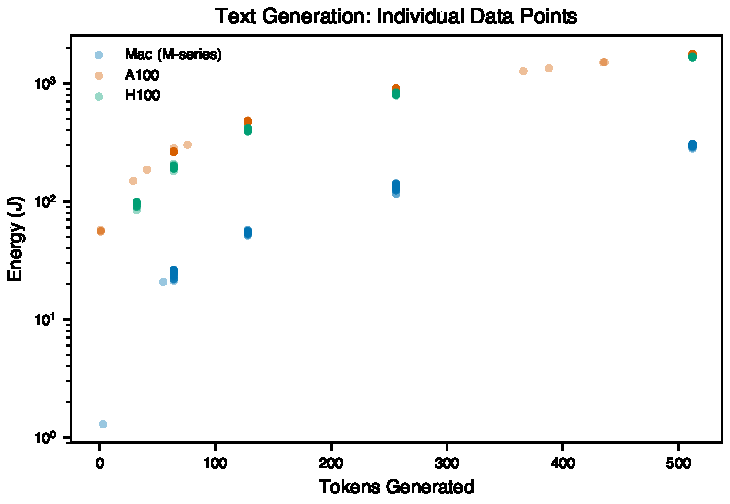
\includegraphics[width=0.85\textwidth]{../figures/supp/supp_fig1_text_scatter.pdf}
\caption{\textbf{Text generation: individual data points.}
All individual energy measurements for text generation using Phi-3-mini-4k across three hardware platforms (Mac M-series, NVIDIA A100, NVIDIA H100). Each point represents a single inference run. The Mac platform shows substantially lower absolute energy consumption at all token counts, while GPU platforms exhibit higher but more consistent energy draw due to high idle power.}
\label{fig:supp1}
\end{figure}

\begin{figure}[H]
\centering
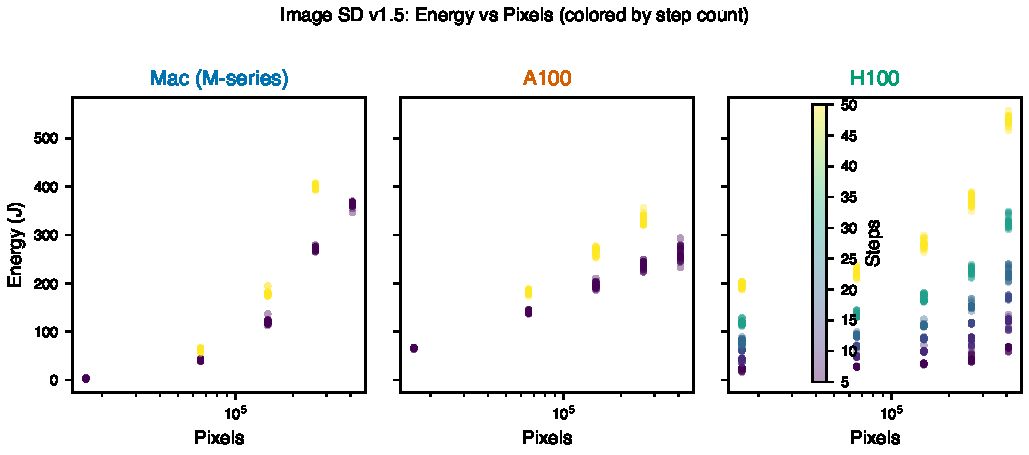
\includegraphics[width=\textwidth]{../figures/supp/supp_fig2_image_scatter.pdf}
\caption{\textbf{Image generation (SD v1.5): individual data points colored by step count.}
Energy consumption for Stable Diffusion v1.5 image generation across all three platforms. Points are colored by the number of diffusion steps. Higher step counts and larger resolutions both increase energy consumption, but the scaling behavior differs markedly between platforms.}
\label{fig:supp2}
\end{figure}

\begin{figure}[H]
\centering
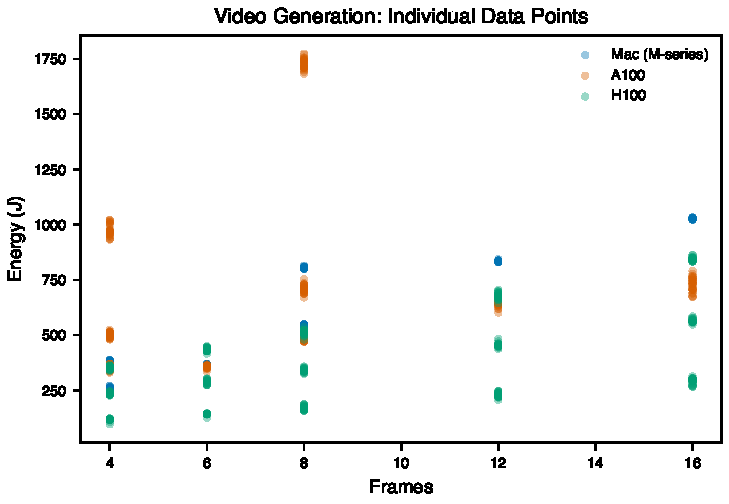
\includegraphics[width=0.85\textwidth]{../figures/supp/supp_fig3_video_scatter.pdf}
\caption{\textbf{Video generation: individual data points.}
All individual energy measurements for AnimateDiff video generation across available platforms. Energy scales with frame count, with the crossover between on-device and cloud efficiency depending on the number of frames generated.}
\label{fig:supp3}
\end{figure}

\begin{figure}[H]
\centering
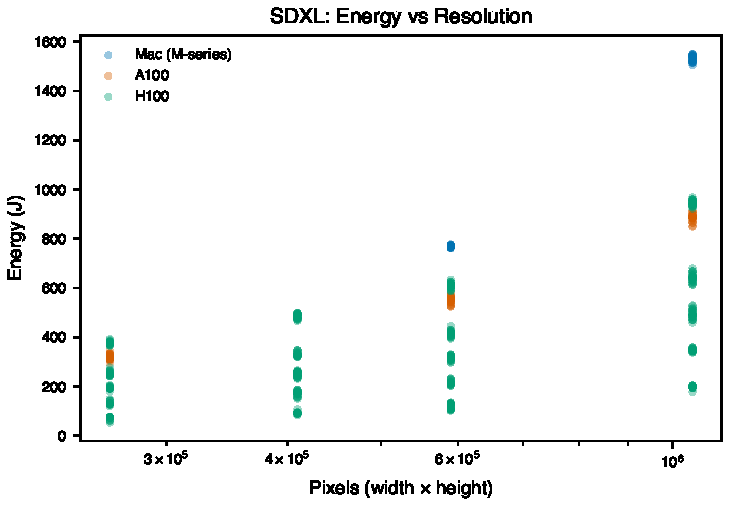
\includegraphics[width=0.85\textwidth]{../figures/supp/supp_fig4_sdxl_scatter.pdf}
\caption{\textbf{SDXL cross-hardware comparison.}
Energy consumption for SDXL image generation across three platforms as a function of output resolution. SDXL requires substantially more compute than SD v1.5, shifting the crossover point to lower resolutions.}
\label{fig:supp4}
\end{figure}

\begin{figure}[H]
\centering
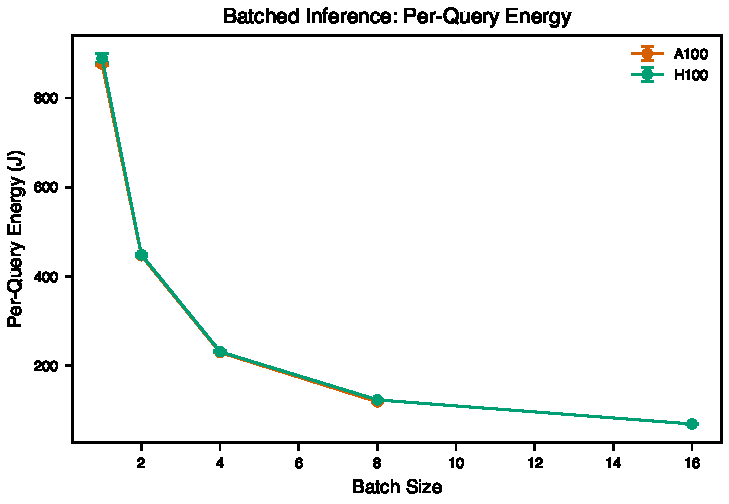
\includegraphics[width=0.85\textwidth]{../figures/supp/supp_fig5_batched.pdf}
\caption{\textbf{Batched inference: per-query energy.}
Per-query energy consumption as a function of batch size for text generation (Phi-3-mini-4k) on A100 and H100 GPUs. Batching amortizes the high fixed power cost of datacenter GPUs, reducing per-query energy. Error bars show $\pm 1$ standard deviation.}
\label{fig:supp5}
\end{figure}

\begin{figure}[H]
\centering
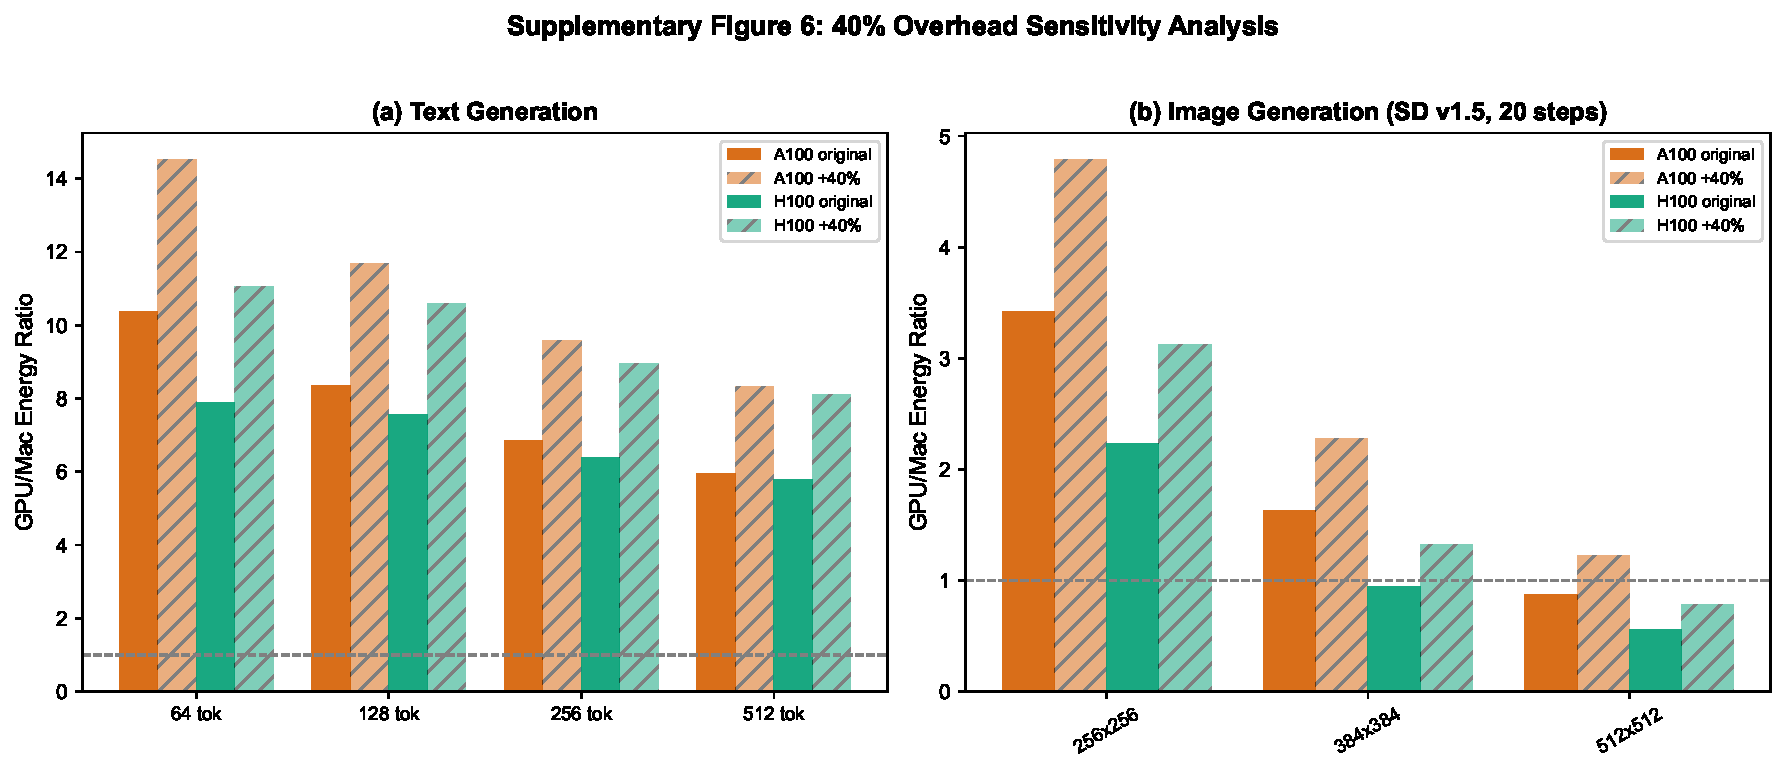
\includegraphics[width=\textwidth]{../figures/supp/supp_fig6_sensitivity.pdf}
\caption{\textbf{Sensitivity analysis: 40\% overhead correction.}
Mac-to-GPU energy ratios before and after applying a 1.4$\times$ multiplier to GPU energy measurements to account for datacenter overhead (cooling, networking, storage). Even with this conservative correction that \emph{reduces} the relative advantage of on-device computing, the crossover effect persists: local inference remains more efficient below the crossover point.}
\label{fig:supp6}
\end{figure}

\begin{figure}[H]
\centering
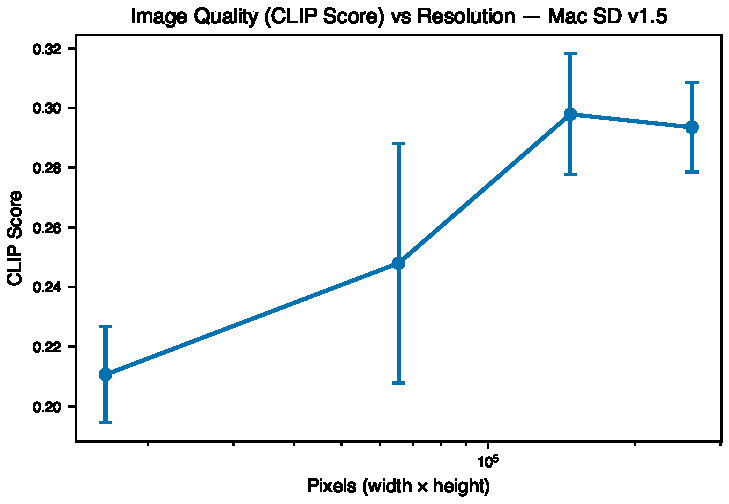
\includegraphics[width=0.85\textwidth]{../figures/supp/supp_fig7_clip_quality.pdf}
\caption{\textbf{Image quality (CLIP score) vs resolution.}
CLIP similarity scores for SD v1.5 generated images as a function of resolution. Quality saturates at moderate resolutions, suggesting that generating at unnecessarily high resolutions wastes energy without meaningful quality improvement.}
\label{fig:supp7}
\end{figure}

\begin{figure}[H]
\centering
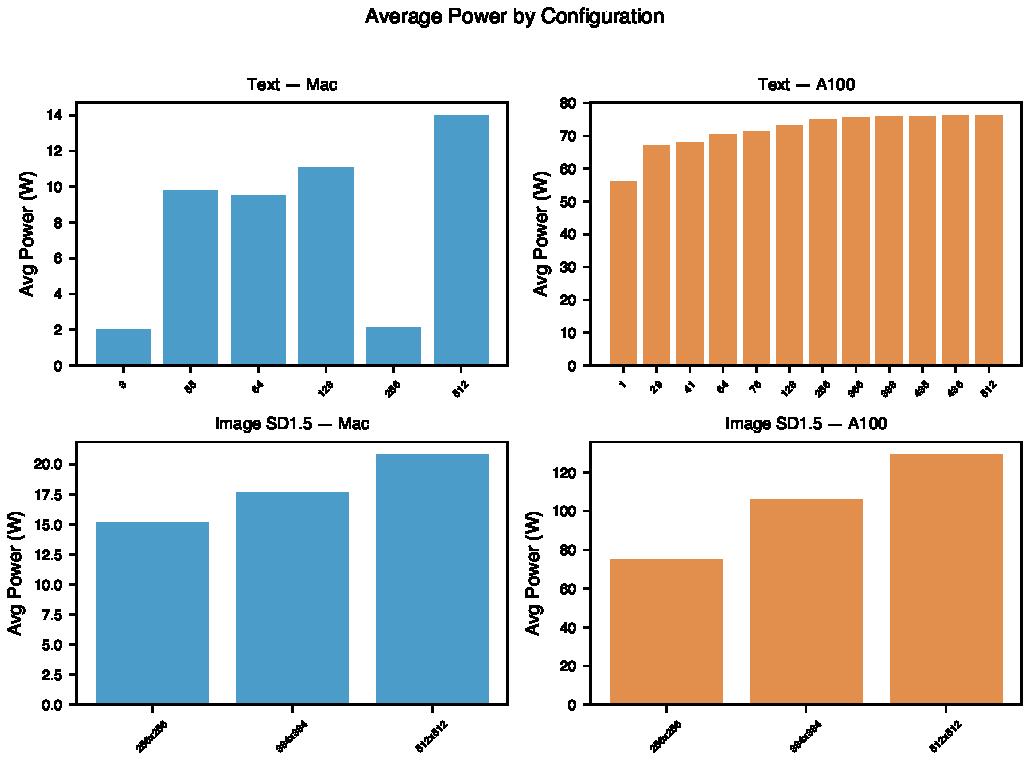
\includegraphics[width=\textwidth]{../figures/supp/supp_fig8_power_traces.pdf}
\caption{\textbf{Average power consumption by configuration.}
Mean power draw (W) for each hardware platform across different generation configurations. Mac devices maintain low power ($\sim$10--30\,W) across all workloads, while datacenter GPUs draw 70--170\,W regardless of task complexity, explaining why they are less efficient for small tasks.}
\label{fig:supp8}
\end{figure}

\begin{figure}[H]
\centering
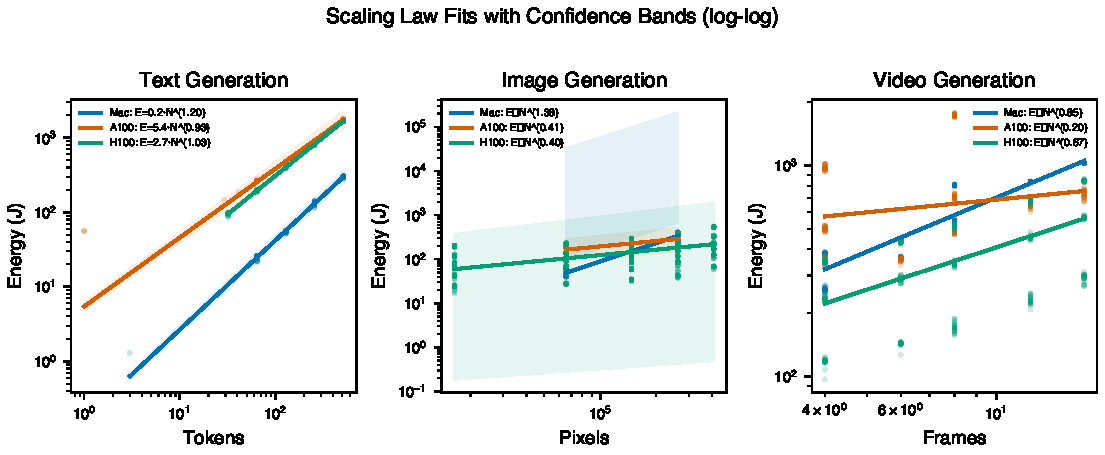
\includegraphics[width=\textwidth]{../figures/supp/supp_fig9_scaling_fits.pdf}
\caption{\textbf{Scaling law fits with confidence bands.}
Log-log plots of energy ($E$) vs output size ($N$) for text (tokens), image (pixels), and video (frames) generation. Lines show power-law fits $E = a \cdot N^b$; shaded regions indicate 1$\sigma$ confidence bands from parameter uncertainty. The Mac exhibits superlinear scaling ($b > 1$) across all modalities, while GPUs show sublinear scaling ($b < 1$) for diffusion workloads (image, video) and near-linear scaling for autoregressive workloads (text), reflecting different hardware utilization regimes.}
\label{fig:supp9}
\end{figure}

\clearpage

%% ================================================================
\section{Supplementary Tables}
%% ================================================================

\subsection{Supplementary Table 1: Per-Configuration Energy Statistics}

\begin{longtable}{llrrrrr}
\caption{\textbf{Complete per-configuration energy statistics.} Mean, standard deviation, minimum, maximum, and number of measurements ($n$) for total energy consumption (J) across all experimental configurations and hardware platforms.} \\
\toprule
Hardware & Configuration & Mean (J) & Std (J) & Min (J) & Max (J) & $n$ \\
\midrule
\endfirsthead
\toprule
Hardware & Configuration & Mean (J) & Std (J) & Min (J) & Max (J) & $n$ \\
\midrule
\endhead
\midrule
\multicolumn{8}{l}{\textbf{Text}} \\
\midrule
Mac & 128 tokens & 53.2 & 6.3 & 20.8 & 57.2 & 30 \\
Mac & 256 tokens & 127.5 & 24.9 & 1.3 & 142.6 & 30 \\
Mac & 3 tokens & 1.3 & 0.0 & 1.3 & 1.3 & 1 \\
Mac & 512 tokens & 288.2 & 54.9 & 0.0 & 307.6 & 30 \\
Mac & 55 tokens & 20.8 & 0.0 & 20.8 & 20.8 & 1 \\
Mac & 64 tokens & 24.5 & 1.6 & 21.2 & 26.3 & 30 \\
A100 & 1 tokens & 56.1 & 0.7 & 55.4 & 57.0 & 3 \\
A100 & 128 tokens & 443.9 & 98.7 & 57.0 & 482.6 & 30 \\
A100 & 256 tokens & 873.9 & 154.6 & 55.8 & 910.2 & 30 \\
A100 & 29 tokens & 148.5 & 0.0 & 148.5 & 148.5 & 1 \\
A100 & 366 tokens & 1266.2 & 0.0 & 1266.2 & 1266.2 & 1 \\
A100 & 388 tokens & 1340.5 & 0.0 & 1340.5 & 1340.5 & 1 \\
A100 & 41 tokens & 185.2 & 0.0 & 185.2 & 185.2 & 1 \\
A100 & 435 tokens & 1502.2 & 0.0 & 1502.2 & 1502.2 & 1 \\
A100 & 436 tokens & 1506.0 & 0.0 & 1506.0 & 1506.0 & 1 \\
A100 & 512 tokens & 1715.1 & 130.3 & 1266.2 & 1779.4 & 30 \\
A100 & 64 tokens & 254.2 & 40.4 & 55.4 & 282.0 & 30 \\
A100 & 76 tokens & 301.2 & 0.0 & 301.2 & 301.2 & 1 \\
H100 & 128 tokens & 402.3 & 7.9 & 388.9 & 417.2 & 30 \\
H100 & 256 tokens & 814.7 & 12.8 & 785.8 & 837.7 & 30 \\
H100 & 32 tokens & 95.4 & 3.5 & 84.4 & 99.1 & 30 \\
\multicolumn{8}{c}{\textit{... 2 more rows ...}} \\
\midrule
\multicolumn{8}{l}{\textbf{Image SD1.5}} \\
\midrule
Mac & 256x256, 20 steps & 41.2 & 1.3 & 38.9 & 44.6 & 30 \\
Mac & 256x256, 30 steps & 62.5 & 2.2 & 55.9 & 67.3 & 30 \\
Mac & 384x384, 20 steps & 120.2 & 4.3 & 113.0 & 137.2 & 30 \\
Mac & 384x384, 30 steps & 178.6 & 4.9 & 173.9 & 194.8 & 30 \\
Mac & 512x512, 20 steps & 272.0 & 3.4 & 265.1 & 278.9 & 30 \\
Mac & 512x512, 30 steps & 399.7 & 3.7 & 392.5 & 407.0 & 30 \\
A100 & 256x256, 20 steps & 141.0 & 2.4 & 136.5 & 145.6 & 30 \\
A100 & 256x256, 30 steps & 182.2 & 3.4 & 174.1 & 188.5 & 30 \\
A100 & 384x384, 20 steps & 196.0 & 5.2 & 185.6 & 210.2 & 30 \\
A100 & 384x384, 30 steps & 267.0 & 6.5 & 253.0 & 277.2 & 30 \\
A100 & 512x512, 20 steps & 238.3 & 6.8 & 223.8 & 249.3 & 30 \\
A100 & 512x512, 30 steps & 333.1 & 8.7 & 320.5 & 356.3 & 30 \\
H100 & 128x128, 10 steps & 42.1 & 2.5 & 35.3 & 45.2 & 30 \\
H100 & 128x128, 15 steps & 62.0 & 1.1 & 60.1 & 64.7 & 30 \\
H100 & 128x128, 20 steps & 79.3 & 4.5 & 70.1 & 89.3 & 30 \\
H100 & 128x128, 30 steps & 119.0 & 4.1 & 111.8 & 129.2 & 30 \\
H100 & 128x128, 5 steps & 23.6 & 2.4 & 16.8 & 26.0 & 30 \\
H100 & 128x128, 50 steps & 196.2 & 5.0 & 187.2 & 203.8 & 30 \\
H100 & 256x256, 10 steps & 48.9 & 0.8 & 47.2 & 50.4 & 30 \\
H100 & 256x256, 15 steps & 69.5 & 2.3 & 58.1 & 72.1 & 30 \\
H100 & 256x256, 20 steps & 92.0 & 2.4 & 88.7 & 99.9 & 30 \\
\multicolumn{8}{c}{\textit{... 21 more rows ...}} \\
\midrule
\multicolumn{8}{l}{\textbf{SDXL}} \\
\midrule
Mac & 1024x1024 & 1531.5 & 12.0 & 1505.7 & 1551.2 & 30 \\
Mac & 512x512 & 315.8 & 2.6 & 309.9 & 320.5 & 30 \\
Mac & 768x768 & 768.6 & 3.8 & 761.2 & 776.9 & 30 \\
A100 & 1024x1024 & 886.5 & 14.5 & 848.6 & 911.8 & 30 \\
A100 & 512x512 & 319.5 & 10.0 & 295.3 & 343.9 & 30 \\
A100 & 768x768 & 552.0 & 13.6 & 524.7 & 583.2 & 30 \\
H100 & 1024x1024 & 525.2 & 257.0 & 177.3 & 968.0 & 150 \\
H100 & 512x512 & 205.0 & 104.8 & 52.6 & 392.4 & 150 \\
H100 & 640x640 & 265.6 & 135.6 & 83.1 & 499.0 & 150 \\
H100 & 768x768 & 334.9 & 169.4 & 101.6 & 633.3 & 150 \\
\midrule
\multicolumn{8}{l}{\textbf{Video}} \\
\midrule
Mac & 12 frames & 834.8 & 2.7 & 829.2 & 843.3 & 30 \\
Mac & 4 frames & 319.8 & 62.0 & 249.1 & 388.1 & 60 \\
Mac & 8 frames & 674.4 & 130.4 & 538.5 & 814.1 & 60 \\
A100 & 12 frames & 648.0 & 18.2 & 601.4 & 678.1 & 30 \\
A100 & 4 frames & 609.0 & 266.3 & 330.7 & 1021.4 & 90 \\
A100 & 8 frames & 975.8 & 539.9 & 470.2 & 1773.5 & 90 \\
H100 & 12 frames & 454.0 & 183.4 & 206.9 & 705.2 & 90 \\
H100 & 16 frames & 566.9 & 225.4 & 265.9 & 863.4 & 90 \\
H100 & 4 frames & 234.3 & 95.8 & 96.6 & 364.6 & 90 \\
H100 & 6 frames & 288.8 & 119.8 & 125.9 & 449.6 & 90 \\
H100 & 8 frames & 340.8 & 139.1 & 156.7 & 535.7 & 90 \\
\midrule
\multicolumn{8}{l}{\textbf{Music}} \\
\midrule
Mac & 11.22s & 139.9 & 0.0 & 139.9 & 139.9 & 1 \\
Mac & 11.26s & 138.1 & 0.0 & 138.1 & 138.1 & 1 \\
Mac & 11.31s & 143.1 & 0.0 & 143.1 & 143.1 & 1 \\
Mac & 11.32s & 141.8 & 0.3 & 141.5 & 142.2 & 2 \\
Mac & 11.44s & 143.4 & 0.0 & 143.4 & 143.4 & 1 \\
Mac & 11.45s & 144.0 & 0.2 & 143.8 & 144.3 & 2 \\
Mac & 11.4s & 143.0 & 0.0 & 143.0 & 143.0 & 2 \\
Mac & 11.56s & 144.7 & 0.0 & 144.7 & 144.7 & 1 \\
Mac & 11.58s & 140.7 & 0.0 & 140.7 & 140.7 & 1 \\
Mac & 11.5s & 143.5 & 0.0 & 143.5 & 143.5 & 1 \\
Mac & 11.61s & 145.2 & 0.0 & 145.2 & 145.2 & 1 \\
Mac & 11.63s & 143.3 & 0.0 & 143.3 & 143.3 & 1 \\
Mac & 11.65s & 145.8 & 0.0 & 145.8 & 145.8 & 1 \\
Mac & 11.69s & 144.4 & 0.0 & 144.4 & 144.4 & 1 \\
Mac & 11.6s & 143.8 & 0.0 & 143.8 & 143.8 & 1 \\
Mac & 11.71s & 145.7 & 0.0 & 145.7 & 145.7 & 1 \\
Mac & 11.72s & 143.2 & 0.0 & 143.2 & 143.2 & 1 \\
Mac & 11.79s & 144.0 & 0.0 & 144.0 & 144.0 & 1 \\
Mac & 11.81s & 143.2 & 0.0 & 143.2 & 143.2 & 1 \\
Mac & 11.83s & 147.1 & 0.0 & 147.1 & 147.1 & 1 \\
Mac & 11.86s & 143.2 & 0.0 & 143.2 & 143.2 & 1 \\
\multicolumn{8}{c}{\textit{... 105 more rows ...}} \\
\midrule
\multicolumn{8}{l}{\textbf{Batched}} \\
\midrule
A100 & batch=1 & 876.1 & 3.2 & 866.7 & 881.9 & 30 \\
A100 & batch=2 & 892.3 & 2.8 & 888.4 & 897.9 & 30 \\
A100 & batch=4 & 917.2 & 3.6 & 909.8 & 924.5 & 30 \\
A100 & batch=8 & 947.6 & 4.1 & 939.4 & 956.7 & 30 \\
H100 & batch=1 & 889.2 & 10.4 & 863.9 & 910.2 & 30 \\
H100 & batch=16 & 1101.0 & 8.7 & 1084.3 & 1120.9 & 30 \\
H100 & batch=2 & 896.7 & 7.7 & 885.6 & 921.5 & 30 \\
H100 & batch=4 & 923.4 & 8.6 & 909.7 & 951.6 & 30 \\
H100 & batch=8 & 983.3 & 10.2 & 964.3 & 1005.4 & 30 \\

\bottomrule
\end{longtable}

\clearpage
\subsection{Supplementary Table 2: Detailed Crossover Analysis}

\begin{table}[H]
\centering
\caption{\textbf{Energy crossover points.} For each modality and platform comparison, we identify adjacent configurations where the Mac-to-GPU energy ratio crosses 1.0 (i.e., where on-device efficiency transitions relative to cloud). Energies are mean values in Joules; the crossover point is linearly interpolated.}
\small
\begin{tabular}{llllllr}
\toprule
Modality & Comparison & Config$_{\text{below}}$ & E (Mac/GPU) & Config$_{\text{above}}$ & E (Mac/GPU) & Crossover \\
\midrule
Image SD1.5 & Mac vs A100 & ('384x384', 30) & 178.6/267.0 & ('512x512', 30) & 399.7/333.1 & 218934 \\

\bottomrule
\end{tabular}
\label{tab:crossover}
\end{table}

\subsection{Supplementary Table 3: Sensitivity Analysis Results}

\begin{longtable}{llrrrrrr}
\caption{\textbf{Sensitivity analysis: original vs 40\%-corrected energy ratios.} GPU energy is multiplied by 1.4$\times$ to account for datacenter overhead. The corrected ratio shows that even with this conservative adjustment, on-device inference remains more efficient for small-to-moderate workloads.} \\
\toprule
Modality & Comparison & Config & Mac (J) & GPU (J) & GPU$_{\text{corr}}$ (J) & Ratio & Ratio$_{\text{corr}}$ \\
\midrule
\endfirsthead
\toprule
Modality & Comparison & Config & Mac (J) & GPU (J) & GPU$_{\text{corr}}$ (J) & Ratio & Ratio$_{\text{corr}}$ \\
\midrule
\endhead
Text & Mac vs A100 & 64 & 24.5 & 254.2 & 355.9 & 0.096 & 0.069 \\
Text & Mac vs A100 & 128 & 53.2 & 443.9 & 621.5 & 0.120 & 0.086 \\
Text & Mac vs A100 & 256 & 127.5 & 873.9 & 1223.5 & 0.146 & 0.104 \\
Text & Mac vs A100 & 512 & 288.2 & 1715.1 & 2401.1 & 0.168 & 0.120 \\
Text & Mac vs H100 & 64 & 24.5 & 193.4 & 270.8 & 0.127 & 0.091 \\
Text & Mac vs H100 & 128 & 53.2 & 402.3 & 563.2 & 0.132 & 0.094 \\
Text & Mac vs H100 & 256 & 127.5 & 814.7 & 1140.6 & 0.156 & 0.112 \\
Text & Mac vs H100 & 512 & 288.2 & 1671.2 & 2339.7 & 0.173 & 0.123 \\
Image SD1.5 & Mac vs A100 & 256x256 & 51.9 & 161.6 & 226.3 & 0.321 & 0.229 \\
Image SD1.5 & Mac vs A100 & 384x384 & 149.4 & 231.5 & 324.1 & 0.645 & 0.461 \\
Image SD1.5 & Mac vs A100 & 512x512 & 335.9 & 285.7 & 399.9 & 1.176 & 0.840 \\

\bottomrule
\end{longtable}

\clearpage

%% ================================================================
\section{Sensitivity Analysis}
%% ================================================================

\subsection{Methodology}

Our primary energy measurements capture GPU-only power consumption via hardware-level power sensors (NVIDIA's \texttt{nvidia-smi} for datacenter GPUs and Apple's \texttt{powermetrics} for M-series chips). However, datacenter GPU deployments incur additional overhead from:

\begin{itemize}
\item \textbf{Cooling infrastructure}: Data centers typically operate at a Power Usage Effectiveness (PUE) of 1.1--1.4, meaning 10--40\% additional energy is consumed for cooling.
\item \textbf{Networking}: Request routing, load balancing, and data transfer consume additional power.
\item \textbf{Storage and memory hierarchy}: Enterprise storage systems and memory management add to the energy budget.
\item \textbf{Redundancy}: Enterprise deployments maintain redundant power supplies and backup systems.
\end{itemize}

To conservatively test the robustness of our crossover findings, we apply a 40\% overhead multiplier ($1.4\times$) to all GPU energy measurements. This represents the upper end of typical PUE values and does \emph{not} include networking or storage overhead, making it a conservative correction that \emph{favors} the GPU side.

\subsection{Results}

As shown in Supplementary Figure~\ref{fig:supp6} and Supplementary Table~3, applying the 1.4$\times$ correction:

\begin{enumerate}
\item \textbf{Reduces} the Mac-to-GPU energy ratio by a factor of 1.4 across all configurations.
\item \textbf{Shifts} the crossover point to somewhat smaller workloads but does \textbf{not eliminate} the crossover effect.
\item Confirms that the fundamental phenomenon---on-device inference being more efficient for small-to-moderate workloads---is robust to reasonable estimates of datacenter overhead.
\end{enumerate}

The persistence of the crossover under this correction strengthens our main finding: the energy advantage of on-device inference for small tasks is a structural property of the hardware power characteristics, not an artifact of measurement methodology.

%% ================================================================
\section{Detailed Scaling Law Fits}
%% ================================================================

We model the energy--output relationship as a power law:
\begin{equation}
E = a \cdot N^b
\end{equation}
where $E$ is total energy (J), $N$ is the output size (tokens for text, pixels for images, frames for video), $a$ is a platform-dependent constant reflecting base power draw and computational overhead, and $b$ is the scaling exponent.

\subsection{Fit Parameters}

\begin{table}[H]
\centering
\caption{\textbf{Power-law fit parameters} $E = a \cdot N^b$ with 1$\sigma$ uncertainties from nonlinear least-squares regression.}
\begin{tabular}{lrr}
\toprule
Configuration & $a$ ($\pm \sigma_a$) & $b$ ($\pm \sigma_b$) \\
\midrule
Text, Mac & 0.1672 $\pm$ 0.0124 & 1.200 $\pm$ 0.012 \\
Text, A100 & 5.4228 $\pm$ 0.5825 & 0.926 $\pm$ 0.018 \\
Text, H100 & 2.6604 $\pm$ 0.0456 & 1.033 $\pm$ 0.003 \\
Image, Mac & 0.0000 $\pm$ 0.0000 & 1.382 $\pm$ 0.032 \\
Image, A100 & 1.8277 $\pm$ 0.5243 & 0.405 $\pm$ 0.024 \\
Image, H100 & 1.1719 $\pm$ 1.4802 & 0.405 $\pm$ 0.102 \\

\bottomrule
\end{tabular}
\label{tab:scaling}
\end{table}

\subsection{Interpretation}

Key observations from the scaling analysis:

\begin{itemize}
\item \textbf{Mac platforms} consistently show $b > 1$ (superlinear scaling) across all modalities, indicating that energy costs grow faster than workload size. This is consistent with memory bandwidth saturation and thermal throttling at higher complexity on the unified memory architecture.
\item \textbf{Datacenter GPUs} (A100, H100) show $b < 1$ (sublinear scaling) for diffusion workloads (image, video), reflecting improving GPU utilization as workload size increases---larger workloads better amortize the high idle power overhead. For autoregressive workloads (text), GPUs show $b \approx 1$ (near-linear scaling) because sequential generation cannot exploit additional parallelism.
\item The \textbf{intercept $a$} is orders of magnitude smaller for Mac platforms, reflecting their fundamentally lower power envelope. This large difference in $a$ is what creates the crossover: at small $N$, the low $a$ of Mac dominates; at large $N$, the more favorable $b$ of GPUs (from parallelism in diffusion workloads) compensates.
\item For \textbf{image generation}, the exponent divergence is most extreme ($b_\text{Mac} = 1.395$ vs $b_\text{A100} = 0.374$), producing the sharpest crossover. The GPU's sublinear scaling reflects the diffusion model's ability to saturate GPU cores at higher resolutions.
\end{itemize}

These fits provide quantitative support for the energy crossover effect: the intersection of two power laws with different $a$ and $b$ parameters creates a natural crossover point whose location depends on the specific hardware and modality combination.

\clearpage
\section*{Supplementary Note 5: Prompt Diversity Analysis}

To validate that energy consumption is determined by computational configuration rather than prompt content, we conducted a prompt diversity experiment using 5 semantically distinct prompts per modality (text and image), each repeated 10 times on the Mac M4 Pro platform.

\textbf{Image generation} shows near-complete prompt invariance: across 5 diverse prompts (landscape, cyberpunk, cat, astronaut, castle) at 512$\times$512 resolution with 20 inference steps, the maximum difference between prompt means was only \textbf{2.0\%} of the overall mean (207.8--211.9~J). The between-prompt variance (2.40) was 13$\times$ smaller than the within-prompt variance (18.15), confirming that run-to-run stochasticity dominates over prompt effects. This is expected because diffusion models execute an identical computational graph regardless of the text conditioning.

\textbf{Text generation} shows slightly higher prompt sensitivity (11.0\% range across prompts at 128 tokens), driven by differences in input tokenization length (7--12 input tokens depending on prompt). However, the between-prompt variance (2.91) remained 14$\times$ smaller than the within-prompt variance (39.54), indicating that measurement noise still dominates. The prompt that produced early termination (38 tokens instead of 128) consumed proportionally less energy (14.6~J vs.\ $\sim$58~J), further confirming that token count, not prompt content, determines energy.

\begin{figure}[H]
\centering
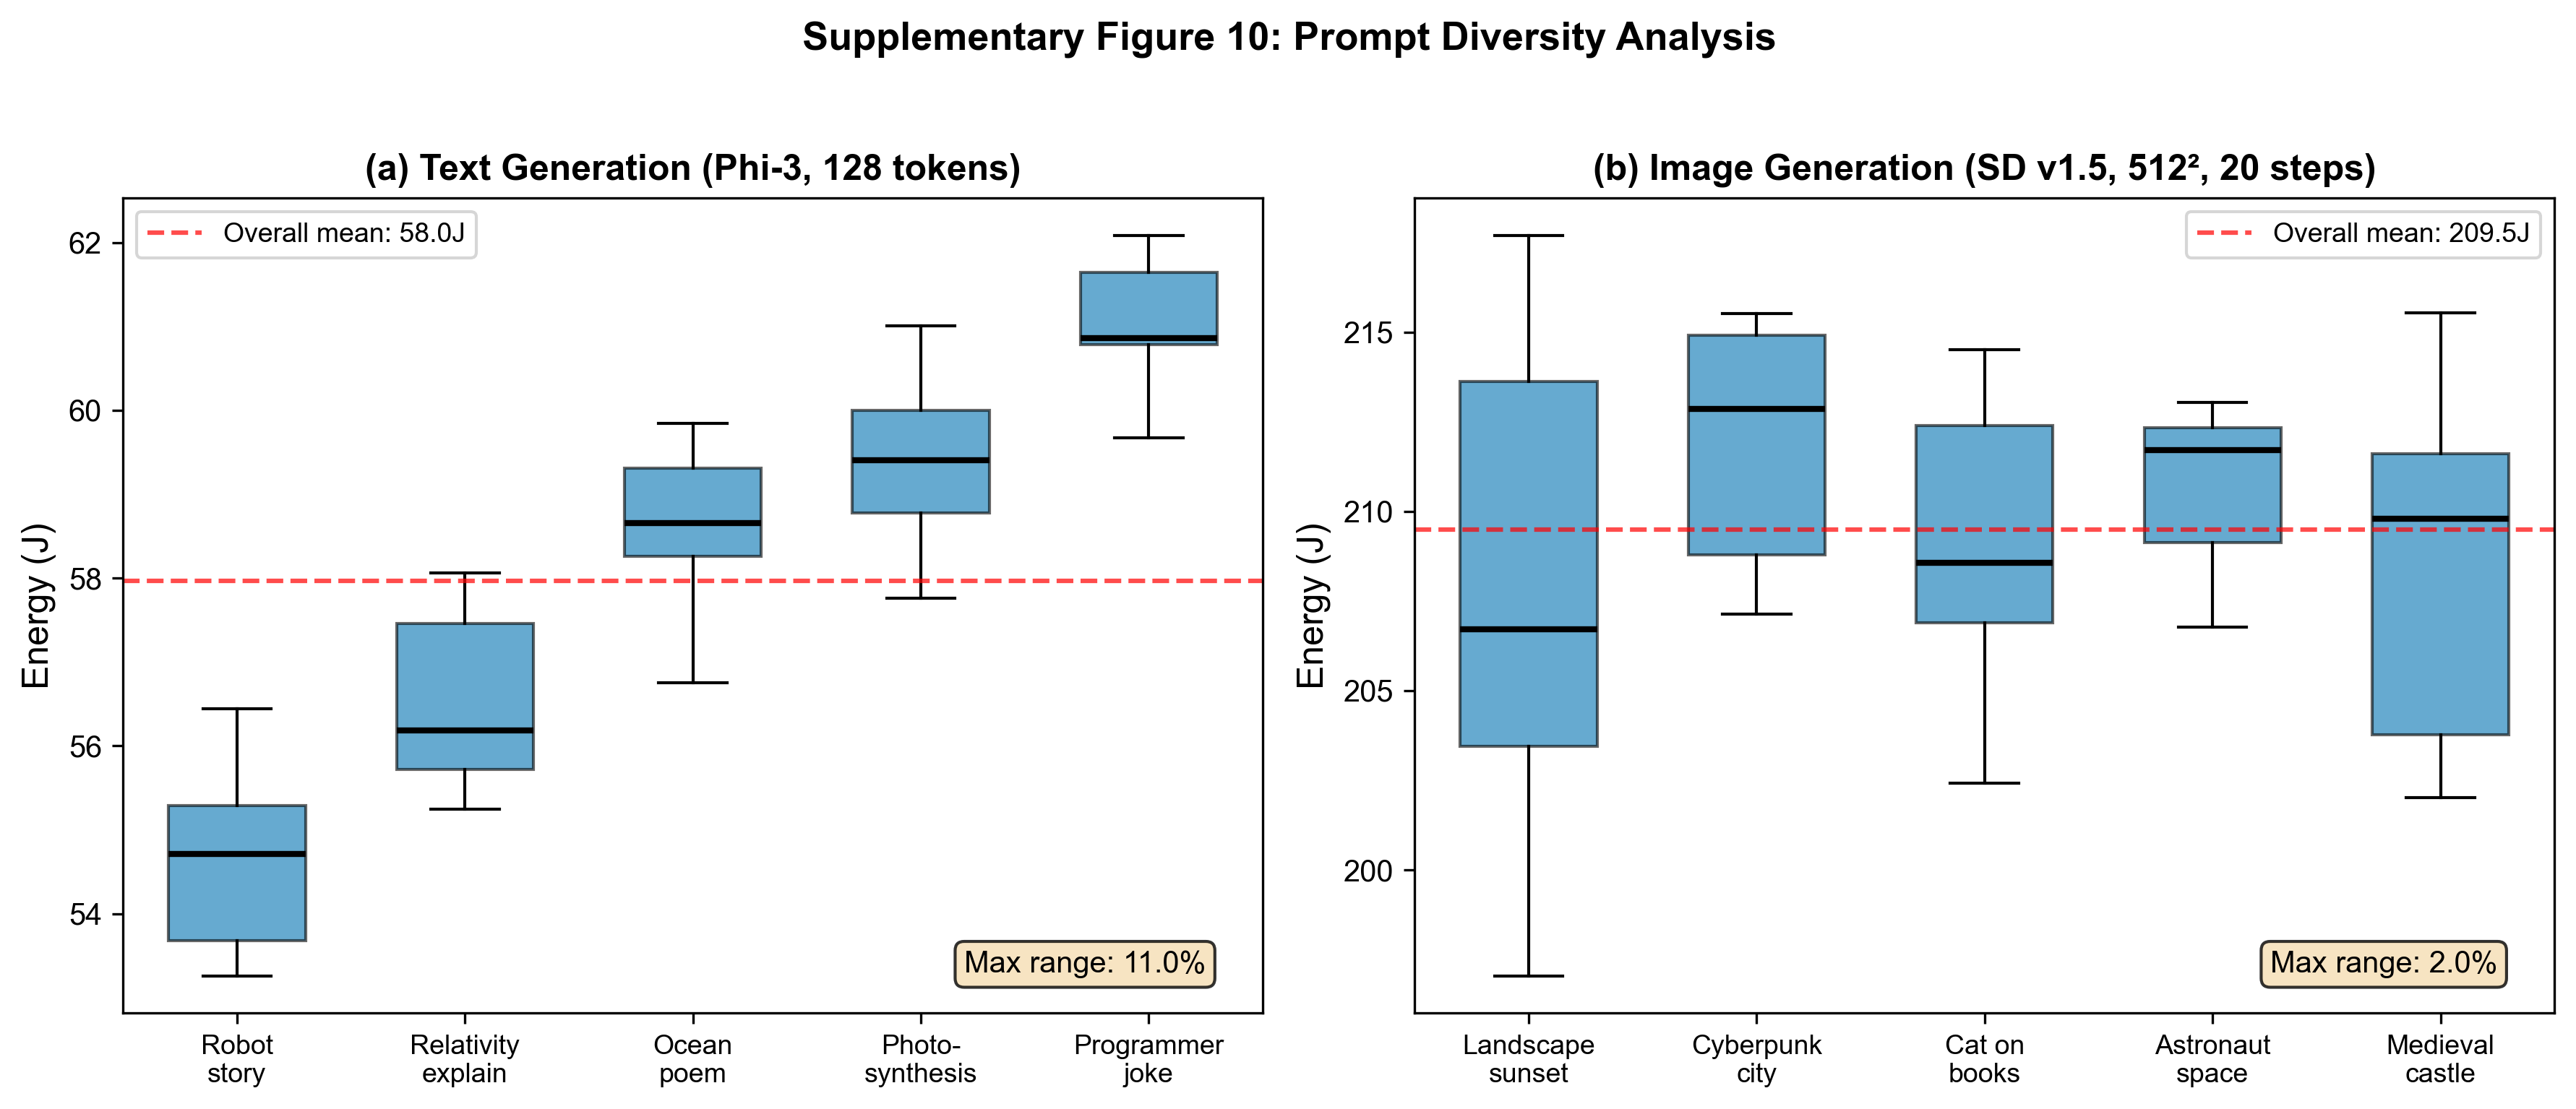
\includegraphics[width=\textwidth]{../figures/supp/supp_fig10_prompt_diversity.png}
\caption{\textbf{Supplementary Figure 10: Prompt diversity analysis.} Box plots showing energy distribution across 5 semantically diverse prompts for (a) text generation (Phi-3, 128 tokens, 128-token runs only) and (b) image generation (SD v1.5, 512$\times$512, 20 steps). Red dashed lines indicate overall means. Maximum between-prompt range is 11.0\% for text and 2.0\% for image, confirming that computational configuration, not prompt content, determines energy consumption.}
\label{fig:prompt_diversity}
\end{figure}

\end{document}
